\section{Stetigähnliche Regler}

Die Stellgrösse $u(t)$ ist noch immer auf wenige Werte beschränkt. \\
Mit den folgenden Konzepten (Abschnitt \ref{Zweipunkteregler mit interner Rückkopplung} und \ref{Schrittregler}) wird aber
erreicht, dass die \textbf{Strecke trotzdem mehr oder weniger 'stetig' beeinflusst} werden kann. \\
\textbf{Gegenüber schaltenden Reglern sind stetigähnliche Regler also aufwendiger zu bauen, aber am Regelausgang ändert sich nicht viel.}

\columnbreak


\subsection{Zweipunkteregler mit interner Rückkopplung}{72}

\label{Zweipunkteregler mit interner Rückkopplung}

\example{$\text{PT}_1$-Glied mit Totzeit als Strecke}

\textbf{Regelinterne Rückkopplung} ($\text{PT}_1$-Glied) zur Reduktion der Schwankungsbreite.
Dieses reagiert ähnlich wie die Strecke, allerdings schneller ($T_r$ klein) und weniger stark \\
($K_r$ gross)

\begin{center}
    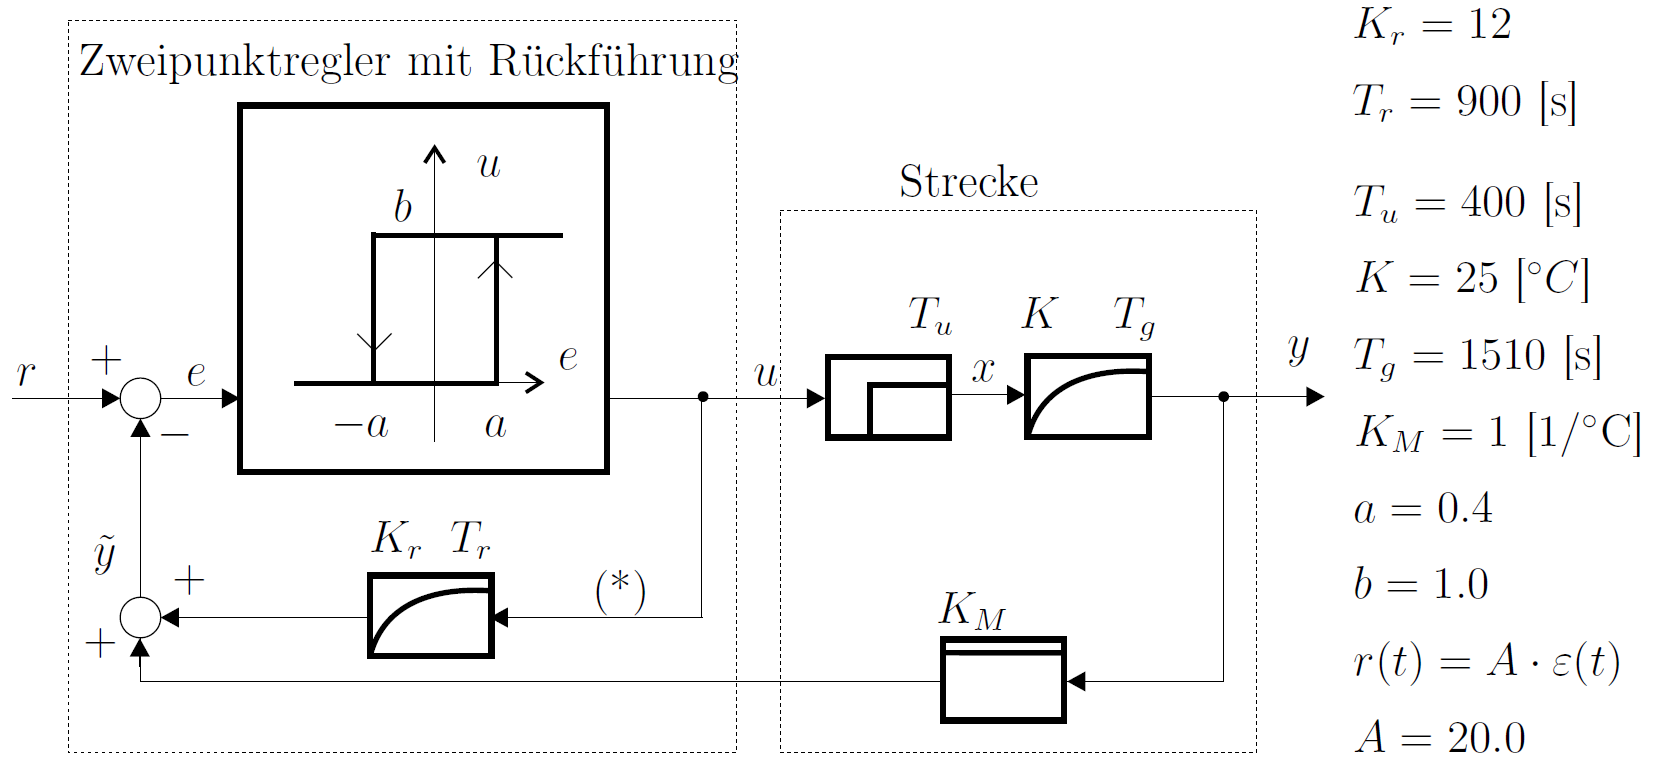
\includegraphics[width=0.8\columnwidth]{images/zweipunkteregler_mit_rueckfuehrung.png}
\end{center}


\textbf{Problem an dieser Schaltung:}

Die Schwankungsbreite ist zwar reduziert, jedoch wird der Sollwert gar nicht erreicht\\
($y_m$ zu tief) \\
Begründung: DC-Verstärkung durch Rückkopplung verändert: 
$$ \tilde{y}_{\rm stat} = (K_M + \frac{K_r}{K}) \cdot y_{\rm stat} \approx 1.5 \cdot y_{\rm stat} $$ 
\textrightarrow\ Dem Regler wird ein zu grosser Messwert geliefert!

\vspace{0.2cm}
\textbf{Alternative:} \\
An der Stelle (*) zusätzlich ein $\text{DT}_1$-Glied einfügen, damit dieser Pfad die DC-Verstärkung Null bekommt.


\subsection{Schrittregler}{74}
\label{Schrittregler}

Häufig befindet sich am Prozesseingang ein Stellantrieb
\vspace{0.1cm}

\textrightarrow\ Fiktive Stellgrösse $v$ kann jeden beliebigen Wert annehmen \\
\textrightarrow\ Regler eher stetig als schaltend 

\begin{center}
    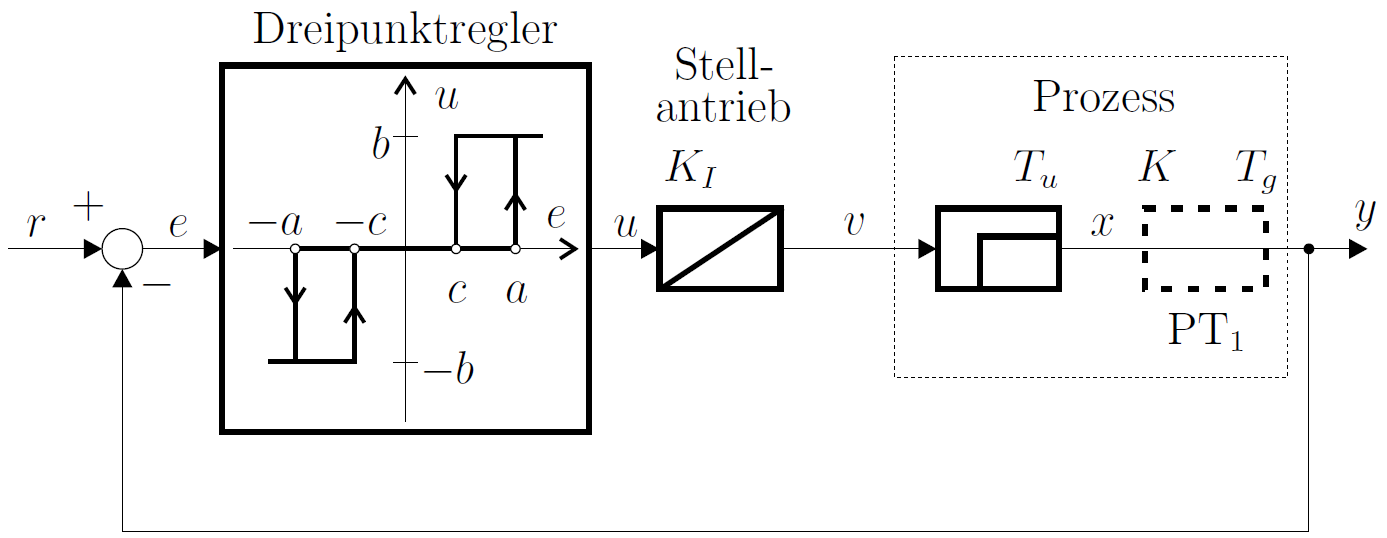
\includegraphics[width=0.8\columnwidth]{images/schrittregler.png}
\end{center}


\example{Stellglied und reiner Totzeit-Prozess (ohne $\text{PT}_1$-Glied)}

$u(t)$ darf nicht erst dann Null gesetzt werden, wenn $y = A$ erreicht wird, da der Prozess noch 'weiterläuft' (Totzeit)

\vspace{0.2cm}

\begin{minipage}{0.44\columnwidth}
    \begin{tabular}{ll}
        $u(t) = b$                      & für $A > a$   \\
        $r(t) = A $                     &               \\
        $v(t) = K_I \, \cdot b \cdot t$ 
    \end{tabular}
\end{minipage}
\hfill
\begin{minipage}{0.55\columnwidth}
    $y(t) =\begin{cases}
    0                               & \text{für } t < T_u   \\
    K_I \, \cdot b \cdot (t - T_u)  & \text{für } t \geq T_u
    \end{cases}$
\end{minipage}

\vspace{0.2cm}

\begin{minipage}{0.65\columnwidth}
    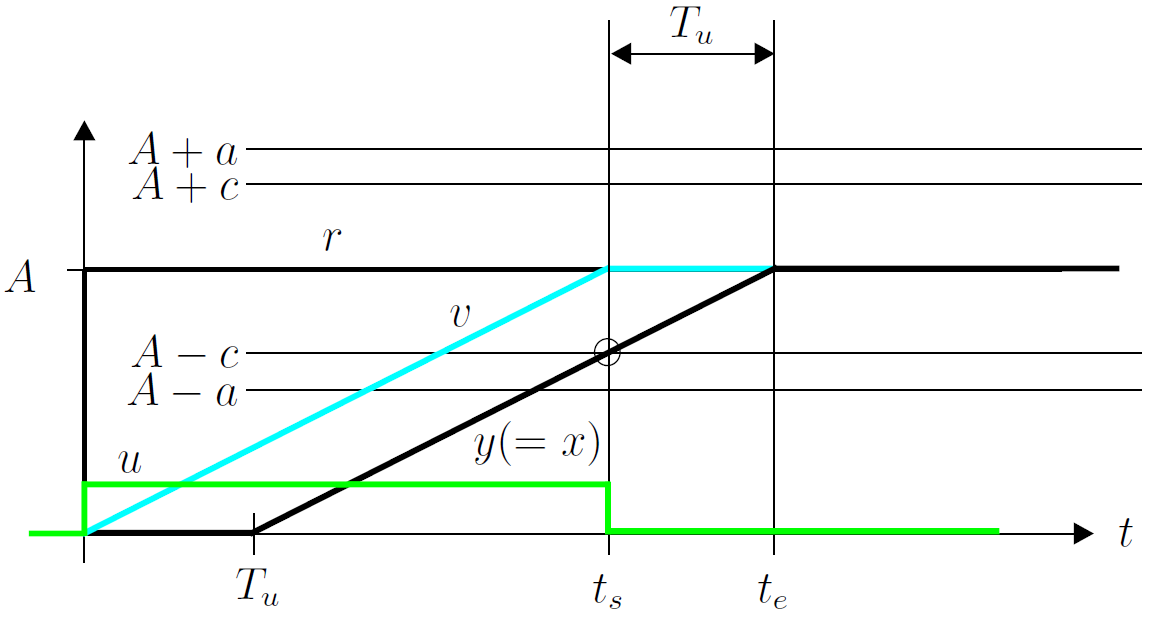
\includegraphics[width=0.9\columnwidth]{images/stellglied_nur_totzeit.png}
\end{minipage}
\hfill
\begin{minipage}{0.32\columnwidth}
    $$ t_e = \frac{A}{K_I \cdot B} + T_u $$
    $$ t_s = t_e - T_u = \frac{A}{K_I \cdot b} $$ 
\end{minipage}

\vspace{0.2cm}
\textbf{Ideale Abschaltzeit $\bm{t_s}$ durch Zurückrechnen finden:} 
$$ y(t_s) = K_I \cdot b \cdot (t - T_u) = A - K_I \cdot b \cdot T_u = A - c $$
$$ \underbrace{ K_I \cdot b}_{\substack{\text{Steigung}}} \cdot T_u = c $$

Parameter $b$ und $c$ auf einander abstimmen, um idealen Ausschaltzeitpunkt zu erreichen

